\section{Results and discussion}

A conventional approach to signal processing and descriptive feature extraction was employed primarily to profile the dataset at hand. However, for the specific task of automatically classifying EEG signals, a more comprehensive, end-to-end deep learning methodology was adopted.


\subsection{Signal processing and feature extraction}
Signal processing and feature extraction are critical steps in EEG analysis since they transform raw, noisy brain activity signals into meaningful representations suitable for interpretation and further analysis. 

EEG signals are complex and susceptible to various artifacts such as muscle movements, eye blinks, and environmental noise, which can obscure the underlying neural information. 

Therefore, processing techniques, such as filtering and artifact removal, help to clean the data and isolate relevant brain activity. Feature extraction, on the other hand, simplifies high-dimensional EEG data by identifying and quantifying key patterns. 

\subsubsection{Filtering}

The data of the EEG signals was first submitted to a band-pass filter, which removed unwanted noise by isolating the frequency range associated with SSVEP stimuli, this being 8-30 Hz. 

Human EEG signals typically range from 1-30 Hz, which is the primary focus of most studies. Low frequency noise appears as slow drifts in the EEG signal over many seconds. In contrast, high frequency noise comes from sources including electromagnetic interference, and muscle contractions (especially facial and neck muscles). High frequency noise looks like spikes in the EEG.

However, since the stimulation frequencies from A Benchmark Dataset for SSVEP-Based Brain-Computer Interfaces ranged from 8-15.8 Hz, the chosen low-cut and high-cut of the band-pass filter were, respectively, set to 7 Hz and 30 Hz.

\subsubsection{Time-Domain Features}

Time-Domain Features, such as Mean (1), Peak-to-Peak Amplitude (2), Peak Amplitude (3) and Variance (4), were extracted from the raw EEG signal over time.
\begin{equation}
  \bar{x} = \frac{1}{n} \sum_{i=1}^{n} x_i   
\end{equation}

\begin{equation}
\text{Peak-to-Peak Amplitude} = \max \left[ x_n \right] - \min \left[ x_n \right]
\end{equation}

\begin{equation}
\text{Peak Amplitude} = \max \left[ x_n \right]
\end{equation}

\begin{equation}
\text{Variance} = \sigma^2 = \frac{1}{n} \sum_{i=1}^{n} \left( x_i - \bar{x} \right)^2
\end{equation}

\begin{figure}[h!]
    \centering
    % Top-left image
    \begin{minipage}[t]{0.45\textwidth}
        \centering
        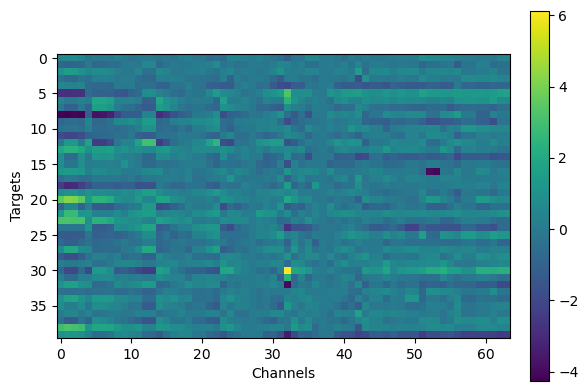
\includegraphics[width=\textwidth]{dtu_logos/mean.png}
        \caption{Mean}
    \end{minipage}
    % Top-right image
    \begin{minipage}[t]{0.45\textwidth}
        \centering
        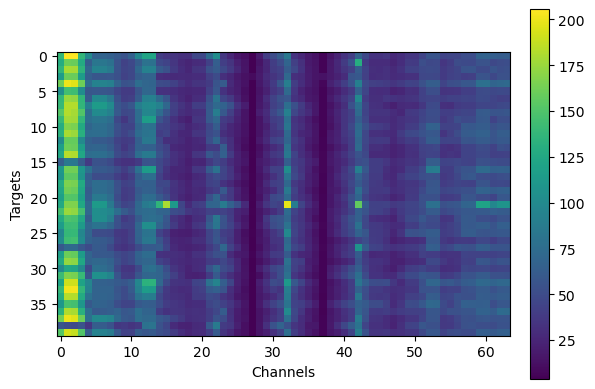
\includegraphics[width=\textwidth]{dtu_logos/ptpa.png}
        \caption{Peak-to-Peak Amplitude}
    \end{minipage}
    
    \vspace{0.5cm}
    
    % Bottom-left image
    \begin{minipage}[t]{0.45\textwidth}
        \centering
        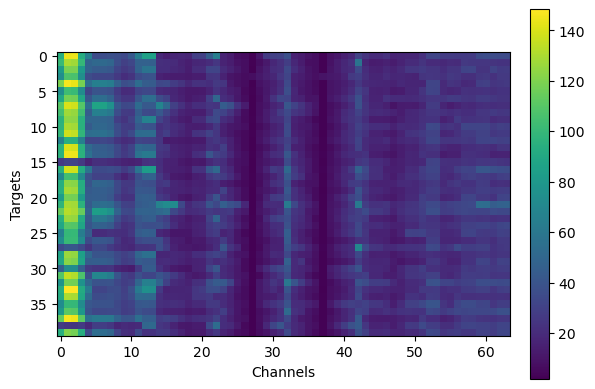
\includegraphics[width=\textwidth]{dtu_logos/pa.png}
        \caption{Peak Amplitude}
    \end{minipage}
    % Bottom-right image
    \begin{minipage}[t]{0.45\textwidth}
        \centering
        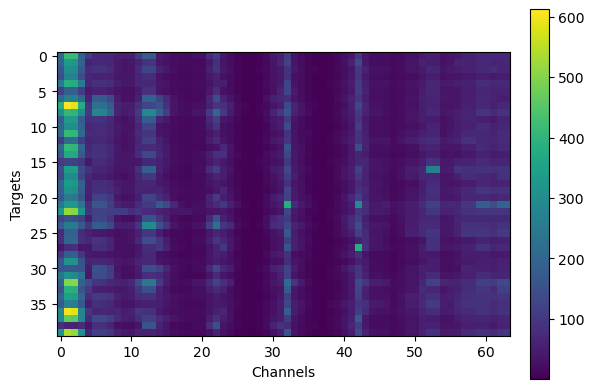
\includegraphics[width=\textwidth]{dtu_logos/variance.png}
        \caption{Variance}
    \end{minipage}
    
    \caption{Time-Domain Features of EEG signals of subject S1, with targets in function of channels}
    \label{fig:2x2grid_simple}
\end{figure}

Figure 5 displays the time-domain features extracted from EEG signals of subject S1, plotted as a function of channels. These features, provide insights into the magnitude, range, and stability of the neural signals during the SSVEP task. Channels with higher values in these metrics indicate stronger or more variable brain activity, which could correspond to regions of interest for classification. 

The channels 59, 60, 62, and 63, located near the occipital region (critical for visual processing), show notable activity. This aligns with the task's focus on visual stimuli, as these areas are predominantly involved in detecting SSVEP responses. Variations in mean amplitude and peak-to-peak values across channels suggest that neural signals are not uniformly distributed, emphasizing the importance of selecting relevant channels for analysis.

\subsubsection{Frequency Domain Features}

For the Frequency Domain Feature extraction, the Power Spectral Density (PSD) was utilized.

PSD measures the power of EEG signals across different frequencies, enabling the identification of dominant components corresponding to visual stimuli. PSD is particularly crucial in SSVEP-based Brain-Computer Interfaces (BCIs) as it highlights power distribution and leverages harmonics to improve detection accuracy.

Additionally, PSD helps evaluate the strength of SSVEP responses under various conditions, making it a reliable tool for feature extraction and performance assessment. By isolating key frequency components, PSD ensures effective and efficient SSVEP detection, which is critical for real-time control and communication tasks.

According, to the analysis by the CNN (see section 4.5) the most relevant channels (i.e. the channels with the biggest weights associated with them) are: 59,60,62 and 63. 

\begin{figure}
    \centering
    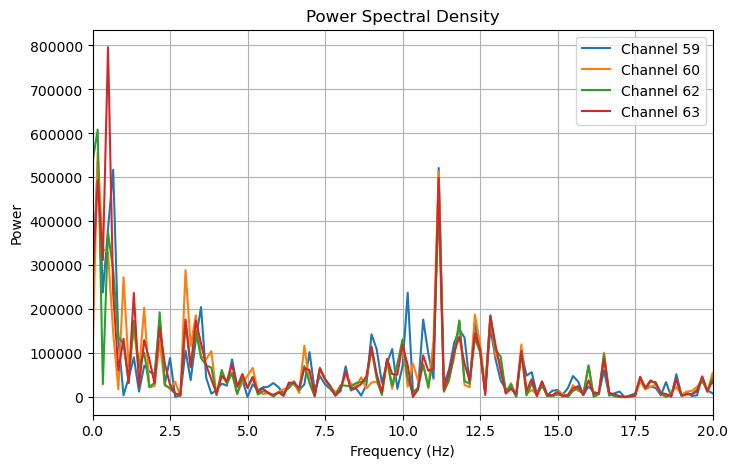
\includegraphics[width=1\linewidth]{dtu_logos/PSD.png}
    \caption{Power Spectral Density of the channels 59,60,62 and 63}
    \label{fig:enter-label1}
\end{figure}

\subsubsection{Time-Frequency Domain Features}

Lastly, the EEG signals of the data set were analyzed using the Wavelet Transform (WT). 

 WT is a crucial tool for time-frequency analysis, offering the ability to decompose EEG signals into time-localized frequency components, which is essential for analyzing non-stationary signals like EEG, where the frequency content changes over time.
 
 WT enables detailed time-frequency localization, allowing the detection of transient features such as SSVEP responses, while its analysis ensures adaptive exploration of low and high-frequency components. This is particularly beneficial for identifying fundamental SSVEP frequencies and harmonics, while minimizing noise interference, thereby improving the signal-to-noise ratio (SNR).

The following figure demonstrates the Raw EGG Signal and its respective Wavelet Transform, for channel=61, target=1, and block=1:

\begin{figure}[H]
    \centering
    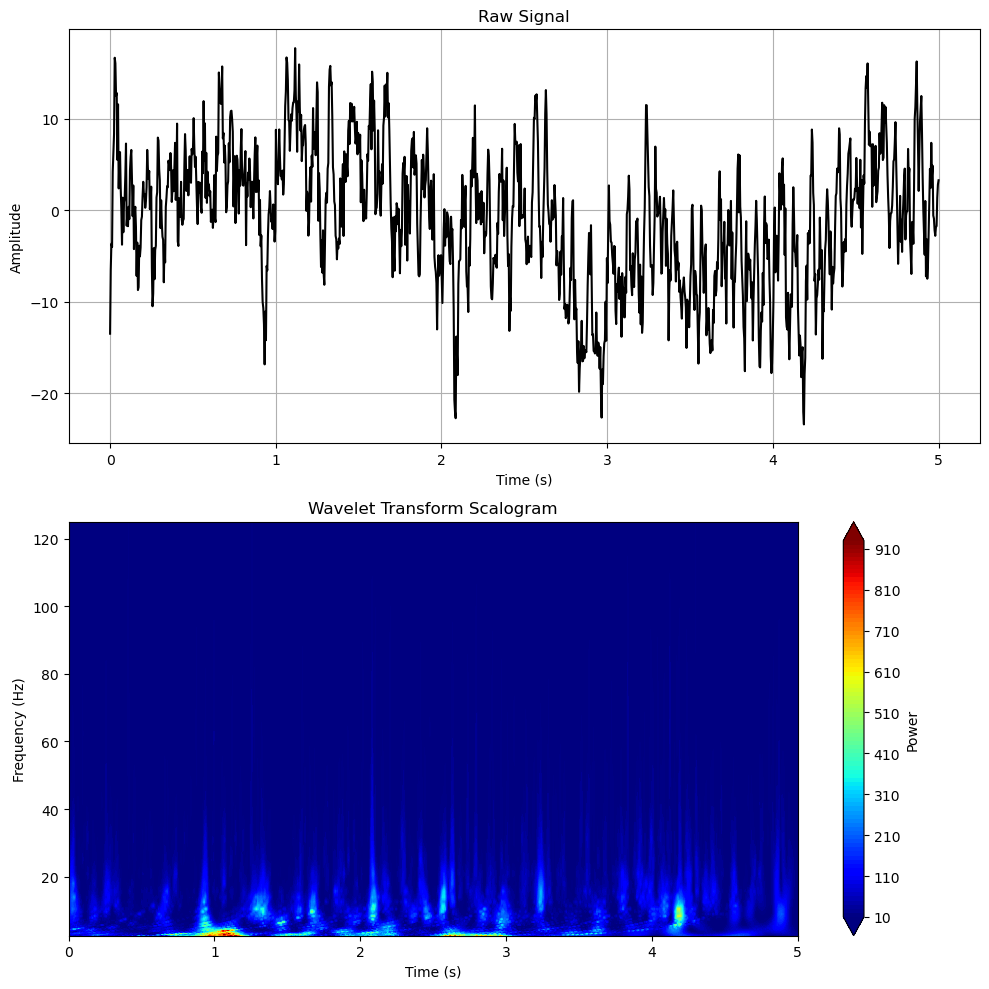
\includegraphics[width=0.75\linewidth]{image.png}
    \caption{Wavelet Transform Scalogram and EEG Raw Signal}
    \label{fig:enter-label2}
\end{figure}

 The scalogram revealed that most of the signal's power is concentrated in the low-frequency range (below 20 Hz), with transient bursts of activity around 1 second and 4 seconds. Minimal high-frequency activity above 40 Hz suggests either preprocessing removed noise or the signal lacks such components. Overall, the scalogram effectively captures the time-frequency dynamics, highlighting dominant frequencies and transient events for further analysis.\cite{cohen2014}\cite{durka2007}

Compared to Fourier-based methods, WT is more effective for analyzing non-stationary signals as its outputs reveal energy distributions across time and frequency, highlighting SSVEP stimulation frequencies and harmonics. This makes 

\subsection{Deep learning}
A more end-to-end, black-box, deep learning approach was taken for the actual task of classification of the signals. The dataset \cite{wang2017benchmark} consisted of 6 trials per target per subject, each trial is 64 channels by 1500 time instants. As said, the task was to develop a classification algorithm to map each trial to the corresponding target the person was looking to.

From the literature, and even though there is no consensus on what the optimal architecture is for each EEG deep learning task, the following points were generally true:
\begin{itemize}
    \item Activation functions - from literature reviews, \cite{xu2023analysis, rakhmatulin2024exploring}, there was no global consensus on what optimal shape function to use, but ReLU, ELU, sigmoid and tanh were the most common, in this order. These introduce non linearity and more expression on the results. ReLU and sigmoid are more prone to gradient vanishing, so ELU was chosen here. % NO CONSESUS ON THE BEST, JUST USE ONE
    \item Dropout - Almost all the models analyzed in \cite{xu2023analysis} used at least one dropout layer, with varying dropout probabilities. Dropout skips some connections and convolutional layers with a certain probability. It can slow down the learning a little bit, but greatly increases the generalization capability of the model, making it perform better on new data.
    \item Batch normalization - the paper in \cite{liu2018deep} first proposed batch normalization layers to greatly increases accuracy of CNNs for EEG P300 tasks. We were also able to prove this for SSVEP (Tab.??, line ??). This is because normalization brings the values of each layer closer to a normal distribution, making it easier for the model to learn.
    \item Augmentation - \cite{lashgari2020data_augment} discusses how data augmentation increases stability, accuracy and reduces overfitting in EEG data. In this study we added Gaussian noise and amplitude scaling data transformations, with a chance of 50\% each.
    \item Pooling - pooling is used to reduce the spacial dimension of the input, reducing the complexity of the learning algorithm. From the literature \cite{xu2023analysis}, both max and average pool were commonly used.
    \item Number of convolutional layers - common literature also uses a range of convolutional layers, from 1 to 4 time convolutions and almost always just one spatial convolutional layer.
    \item Kernel dimensions - Small kernels allow the network to learn small local changes, and larger kernels infer on more global features. According to \cite{xu2023analysis}, the preferred kernel size from the literature is less than $1 \times 25$. Bigger kernels were used and reported here if for some reason they provided better results.
    \item Optimizer, regularization and learning rate - from \cite{xu2023analysis}, the most used optimizer is still Adam (with gradient descent and stochastic gradient descent as runner ups). A base learning rate of $10^-3$ was used, and the $\lambda$ parameter for the L2 regularization (\textit{weight\_decay} in Torch) was set to 0.05.
\end{itemize}


We were able to test most of these with ablation studies on our proposed network to validate the impact of each of the components on the machine learning result. However, the optimal set of hyper parameters for each machine learning task is generally a result of trial and error, following good machine learning practices, with some lucky guesses.



\subsection{Architecture}
\begin{figure}[H]
    \centering
    \includegraphics[width=0.45\linewidth]{Images/Frame 7.png}
    \caption{Schema for the proposed network architecture, with general parameters ($W_i$=size of kernel $i$, $F_i$=number of channels of convolution $i$, $P$=size of pool kernel)}
    \label{fig:architecture}
\end{figure}

Before arriving at the final architecture, a lot of alternative networks were tested. These were directly proposed from other works, adaptations from those, or proposed by generative AI. The results from these won't be reported, as they were worse and harder to fine-tune.
Based in the literature mentioned before, performing some modifications or rewriting new CNN architectures, the final proposed architecture was derived (Fig \ref{fig:architecture}), and implemented in Pytorch. This network is totally end-to-end, with no preprocessing, and mostly inspired by \cite{schirrmeister2017deep}, with one less block. It has a very general architecture of 1 temporal convolution, one depthwise spatial convolution, 2 more depthwise temporal convolutions, and a total of 3 pool layers, plus activations, dropout and batch normalization layers, with a final block with 2 options, that will be explained further. The network has a lot of customizable parameters used for hyperparameter fine-tuning, like the size of convolutional and pool kernels, number of channels and the padding.

Regarding the final block, the result from the convolutional layers can be processed in 2 different ways to predict the final classes. The first option consists of a simple fully connected linear layer followed (or not) by a softmax activation (to turn the predictions into probabilities). This is a very common approach in literature, and was also done by \cite{schirrmeister2017deep}.

The second approach, inspired by \cite{khok2020deep_goncalo} used a final convolutional layer (network with no linear layers), that applies one depthwise kernel on the \textbf{entirety} of the previous layer's results per each class. This maps a shape of $F_4\times1\times46$ directly into a $F_4\times1\times46$ $N_{classes} \times1\times1$ vector, used directly for the prediction of the class. This approach used in \cite{khok2020deep_goncalo} was for multi-target classification on the same dataset, but it actually proved to have the really good results in our classification task.


%EXPLICAR AS DUAS OPCOES E A ARCHITETURA MELHOR


%\subsection{Implementation and training}


\subsection{Training and results}
The proposed network options were trained for 20 epochs, with only 10 subjects data (due to lack of disk space to run with every subject). With this, we had 2400 trials, with 6 trials per patient per class. A 80-20 train-validation split was performed for the training setup, with a batch size of 16.
Data augmentation was preformed: when loading a trial for training, there is a 50\% chance of including Gaussian noise or amplitude scaling.
Training was performed on DTU's High Performance Computing cluster (HPC), with GPU acceleration and CUDA support.

Training and validation accuracy results from training the network with different parameters are shown in tables \ref{tab:cnn_results1} and \ref{tab:cnn_results2}.

% BEST MODEL FOR EACH OPTION
For the first option, a setting with a $1\times2$ pool, padding set to "same" and convolutional kernels of roughly $1/10$ the size of that layer achieved better results.
For the second option for the last block, a pool kernel of size 1 (meaning no pool is performed, like in \cite{khok2020deep_goncalo}), with smaller number of channels (small F1, F2, F3 and F4) and small kernels (small W1, W2 and W3) provided better results. Interestingly, this setup uses less weights (10 times less parameters than the best model found for option 1), but achieves very similar results and really good generalization capabilities and relatively fast learning \ref{}.

% WHAT IMPACTS THE MODEL THE MOST
Changing the pool size, dropout rate and the inclusion of batch normalization layers had a big impact on the performance for both options. The number of out channels in the last layer (F4) and the type of padding ("valid" or "same") also impacted the results, to a lesser extent.
For both options, the huge majority of the model's parameters are concentrated on the last block, either in the fully connected or the convolutional layer.




\begin{table}[ht]
\centering
\resizebox{\textwidth}{!}{
\begin{tabular}{@{}ccccccccccccccc@{}}
%\begin{tabular}{@{}c>{\rowmac}c>{\rowmac}c>{\rowmac}c>{\rowmac}c>{\rowmac}c>{\rowmac}c>{\rowmac}c>{\rowmac}c>{\rowmac}c>{\rowmac}c>{\rowmac}c>{\rowmac}c>{\rowmac}c>{\rowmac}c>{\clearrow}@{}}
Model & $F_1$ & $F_2$ & $F_3$ & $F_4$ & $W_1$ & $W_2$ & $W_3$ & Pool & Dropout & Padding & \# Parameters & \begin{tabular}[c]{@{}c@{}}Training\\ Accuracy\end{tabular} & \begin{tabular}[c]{@{}c@{}}Validation\\ Accuracy\end{tabular} & ITR \\ \midrule
1 & 10 & 20 & 40 & 80 & 39  & 19 & 19 & 2 & 0.5   & same  & 503,490 & 100.00\% & 95.21\% & 57.49 \\
1 & 10 & 20 & 40 & 80 & 121 & 59 & 19 & 2 & -   & same  & 505,910 & 100.00\% & 96.25\% & 58.72 \\
1 & 10 & 20 & 40 & 80 & 121 & 59 & 11 & 2 & -   & same  & 505,270 & 100.00\% & \textbf{97.50\%} & 60.25 \\
1 & 10 & 20 & 40 & 80 & 121 & 59 & 11 & 2 & -   & same  & 504,970 & 100.00\% & 93.75\% & 55.85 \\
1 & 10 & 20 & 40 & 80 & 124 & 61 & 31 & 2 & -   & \textbf{valid} & 359,780 & 100.00\% & 94.17\% & 56.31 \\
1 & 10 & 20 & 40 & 40 & 124 & 61 & 31 & 2 & -   & same  & 256,180 & 100.00\% & 96.88\% & 59.47 \\
1 & 5  & 10 & 20 & 40 & 124 & 61 & 31 & 2 & -   & same  & 249,640 & 100.00\% & 96.46\% & 58.97 \\
1 & 10 & 20 & 40 & 80 & 61  & 61 & 19 & 2 & -   & same  & 505,390 & 100.00\% & 95.63\% & 57.98 \\
1 & 10 & 20 & 40 & 80 & 31  & 31 & 19 & 2 & -   & same  & 503,890 & 100.00\% & 96.46\% & 58.97 \\
1 & 10 & 20 & 40 & 80 & 124 & 41 & 13 & \textbf{3} & -   & same  & 152,740 & 95.31\%  & 15.83\% & 2.92  \\
1 & 10 & 20 & 40 & 80 & 39  & 19 & 19 & \textbf{3} & -   & same  & 151,490 & 85.42\%  & 15.42\% & 2.77  \\
1 & 20 & 20 & 40 & 80 & 59  & 19 & 19 & \textbf{3} & -   & same  & 120,300 & 69.38\%  & 7.08\%  & 0.50  \\
1 & 10 & 20 & 40 & 80 & 39  & 19 & 19 & \textbf{4} & - & same  & 65,080  & 53.12\%  & 6.04\%  & 0.32  \\
1 & 10 & 20 & 40 & 80 & 39  & 11 & 5  & \textbf{4} & -   & same  & 63,650  & 39.38\%  & 5.63\%  & 0.26  \\ \bottomrule
\end{tabular}}
\caption{Summary of CNN model configurations and accuracy results for option 1 with best model}
\label{tab:cnn_results1}
\end{table}



\begin{table}[ht]
\centering
\resizebox{\textwidth}{!}{
\begin{tabular}{@{}ccccccccccccccc@{}}
%\begin{tabular}{@{}c>{\rowmac}c>{\rowmac}c>{\rowmac}c>{\rowmac}c>{\rowmac}c>{\rowmac}c>{\rowmac}c>{\rowmac}c>{\rowmac}c>{\rowmac}c>{\rowmac}c>{\rowmac}c>{\rowmac}c>{\rowmac}c>{\clearrow}@{}}
Model & $F_1$ & $F_2$ & $F_3$ & $F_4$ & $W_1$ & $W_2$ & $W_3$ & Pool & Dropout & Padding & \# Parameters & \begin{tabular}[c]{@{}c@{}}Training\\ Accuracy\end{tabular} & \begin{tabular}[c]{@{}c@{}}Validation\\ Accuracy\end{tabular} & ITR \\ \midrule
2 & 5 & 5 & 5 & 40 & 101 & 19 & 19 & 1 & 0.5 & valid & 46,350 & 99.90\% & 96.04\% & 58.47 \\
2 & 5 & 5 & 5 & 40 & 59 & 19 & 19 & 1 & - & valid & 47,820 & 99.79\% & 96.25\% & 58.72 \\
2 & 5 & 5 & 10 & 40 & 101 & 19 & 19 & 1 & - & valid & 46,455 & 99.84\% & \textbf{96.67\%} & 59.22 \\
2 & 5 & 10 & 20 & 40 & 59 & 19 & 19 & 1 & - & valid & 48,465 & 99.90\% & 95.42\% & 57.74 \\
2 & 10 & 20 & 40 & 80 & 59 & 19 & 19 & 1 & - & valid & 96,930 & 99.95\% & 93.75\% & 55.85 \\
2 & 10 & 20 & 40 & 80 & 101 & 19 & 19 & 1 & - & valid & 93,990 & 99.90\% & 94.38\% & 56.55 \\
2 & 10 & 20 & 40 & 80 & 101 & 39 & 19 & 1 & - & valid & 93,190 & 99.43\% & 94.17\% & 56.32 \\
2 & 20 & 40 & 80 & 160 & 59 & 19 & 19 & 1 & - & valid & 193,860 & 98.96\% & 88.75\% & 50.64 \\
2 & 5 & 10 & 20 & 40 & 59 & 19 & 19 & \textbf{2} & - & valid & 7,625 & 38.39\% & 30.41\% & 9.09 \\ \bottomrule
\end{tabular}}
\caption{Summary of CNN model configurations and accuracy results for option 2 with best model}
\label{tab:cnn_results2}
\end{table}
\vspace{-0.5cm}

%PLOT ACCURACY VS NUMBER OF PARAMETRS FOR EACH ??

%PLOT ACCURACY VS EPOCH

\begin{figure}[H]
    \centering
    % Top-left image
    \begin{minipage}[t]{0.45\textwidth}
        \centering
        \includegraphics[width=\textwidth]{Images/Train curves opt1.png}
        \caption{Option 1}
    \end{minipage}
    % Top-right image
    \begin{minipage}[t]{0.45\textwidth}
        \centering
        \includegraphics[width=\textwidth]{Images/Train curves opt2.png}
        \caption{Option 2}
    \end{minipage}
    \vspace{-0.2cm}
    
    \caption{Training curves for the best parameter for both options}
    \label{fig:trainingcurves}
\end{figure}
\vspace{-0.5cm}



%As is clear from the table \ref{}, the results with option 2 were overwhelmingly better, for every combination of hyperparameters. 

The learning curves for the best model for both options (Fig.\ref{fig:trainingcurves}.a and Fig.\ref{fig:trainingcurves}.b) also demonstrate a lack of overfitting, as the training and validation accuracies in each epoch go up steadily. For option 1, with considerably more parameters, the accuracies rose very fast: after 5 epochs the training accuracy was already above 99\%. Both accuracies plateaued after 10 epochs for these models, with the validation accuracy staying consistently below the training accuracy.

% 11th subject
Finally, we evaluated the best model of both options against a 11th subject's data that wasn't used for training. They both reported an accuracy of 95\% on this data, further confirming the lack of overfitting and the ability to classify and generalize the learning process.


\subsection{Visualizing weights}
In this section, we developed another Python script to load the trained models, extract the learned weights on each layer and visualize them. 

\begin{figure}[H]
    \centering
    \includegraphics[width=0.75\linewidth]{Images/W1_opt1.png}
    \caption{Weights for the first temporal layer for the best setup of option 1}
    \label{fig:W1}
\end{figure}


\begin{figure}[H]
    \centering
    \includegraphics[width=0.6\linewidth]{Images/W2_opt1.png}
    \caption{Weights for the first depthwise spatial layer for the best setup of option 1}
    \label{fig:W2}
\end{figure}


\begin{figure}[H]
    \centering
    \includegraphics[width=0.6\linewidth]{Images/BarcodeW2_opt1.png}
    \caption{Mean of the absolute values for the weights of the first depthwise spatial layer, for the best setup of option 1}
    \label{fig:W2_barcode}
\end{figure}

Fig.\ref{fig:W1} shows the learned weights for the first temporal convolution in the best setup for option 1. Each row represents a kernel.  
Fig.\ref{fig:W2} shows the learned weights for the first depthwise convolution. Then, Fig.\ref{fig:W2_barcode} shows the mean of the absolute value of these weights for each channel, in a barcode format. This plot allows us to pinpoint which electrode channel the model pays more attention to. From that, electrodes 59, 60, 62 and 63, with 62 being exceptionally strong. These correspond to electrodes PO8, CB1, Oz and O2 respectively, all on the occipital region, which is responsible for visual perception in the brain. This is a very relevant finding, as it demonstrates that even without imputing prior knowledge of how the brain functions (by only using the signals from the electrodes in the occipital region for the classification, for example), the network is able to learn that on its own. It's hard to draw conclusions from the weights of the other layers, as there is no apparent pattern in them, so they wont be shown.
Aditionally, the weights visualized and conclusions were very similar for the second architecture option. 